%
%  untitled
%
%  Created by Asger Pedersen on 2012-01-04.
%  Copyright (c) 2012 . All rights reserved.
%
\documentclass[]{article}

% Use utf-8 encoding for foreign characters
\usepackage[utf8]{inputenc}

% Setup for fullpage use
\usepackage{fullpage}

\usepackage{hyperref}
\usepackage{pdfpages}
% Uncomment some of the following if you use the features
%
% Running Headers and footers
%\usepackage{fancyhdr}

% Multipart figures
%\usepackage{subfigure}

% More symbols
%\usepackage{amsmath}
\usepackage{amssymb}
%\usepackage{latexsym}

% Surround parts of graphics with box
\usepackage{boxedminipage}

% Package for including code in the document
\usepackage{listings}

% If you want to generate a toc for each chapter (use with book)
\usepackage{minitoc}

% This is now the recommended way for checking for PDFLaTeX:
\usepackage{ifpdf}

%\newif\ifpdf
%\ifx\pdfoutput\undefined
%\pdffalse % we are not running PDFLaTeX
%\else
%\pdfoutput=1 % we are running PDFLaTeX
%\pdftrue
%\fi

\usepackage{ifpdf}
\title{ Project Course: Development Studio \\ Deliverable 5: Sprint \#4}
\author{ Asger Pedersen, Kristoffer Cobley, Hari Charan \& Jesper Tved }
\setlength{\parindent}{0pt}
\setlength{\parskip}{2ex}
\linespread{1.3}

\begin{document}

\ifpdf
\DeclareGraphicsExtensions{.pdf, .jpg, .tif}
\else
\DeclareGraphicsExtensions{.eps, .jpg}
\fi

\maketitle
\setcounter{tocdepth}{1}
\tableofcontents
\newpage
\section{Sprint Material} % (fold)
\label{sec:Sprint Material}
\subsection{Version} % (fold)
\label{sub:Version}
The current state of our app has version 0.0.1. Meaning that the app is still alpha quality, with some functionality implementet, but lot of unfinished work.
% subsection Version (end)
\subsection{Source code} % (fold)
\label{sub:Source code}
We still use Git and GitHub. The source code is available at: \verb!https://github.com/mundane/ETA_analytics!, in the app folder. The other folders contains prototypes and experiments.
% subsection Source code (end)
\subsection{Sprint Explanation}
The burndown chart shows that, in spite of exams and easter holidays stalled the progress of development in the beginning of the sprint, we did manage to finish some of the tasks within the sprint time frame.
\begin{figure}[h!]
  \centering
    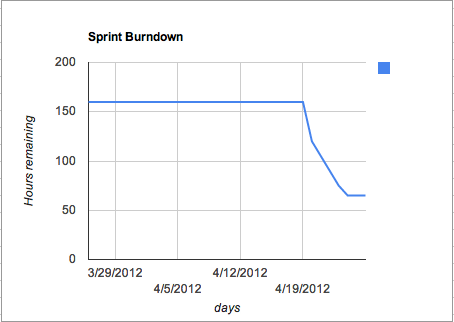
\includegraphics[width=0.8\textwidth]{images/burndown.png}
	\caption{Burndown chart for sprint \# 2. Easter holidays and exams is the reason for the steep curve.}
\end{figure}

\subsection{User Stories}
For sprint \# 2 we had the following user stories: \\
As an analytic \\
I want to make pie charts, column charts, bar charts, etc \\
So that I can make data more presentable \\

As an analytic \\
I want to make charts interactive  \\
So that I can make data more presentable \\

As an analytic \\
I want a way to show selected data from the chart \\
So that I can make data more presentable\\

As an analytic \\
I want to save data for later sessions \\
So I can continue working on datasets \\

\subsection{Tasks} % (fold)
\label{sub:Tasks}
We divided the stories up in the following tasks
% subsection Tasks (end)Tasks
\begin{itemize}
	\item Read up on the MVC model
	\item Research testing tools for Sencha
	\item Research JSLint
	\item Convert CSV format to JSON
	\item Create datagrid from JSON
	\item Make integration to Jstat in the datagrid view
	\item Create charts
\end{itemize}










% section Sprint Material (end)


\section{Sprint Retrospective} % (fold)
\label{sec:Sprint Retrospective}

% section Sprint Retrospective (end)

\section{Process improvements} % (fold)
\label{sec:improvements}
To do process improvements, we had to investigate our existing processes. We looked at our earlier sprint retrospectives, to see what issues we had experienced before.
\begin{itemize}
	\item We underestimated the time needed for many tasks, often because we had no prior experience with the subject and therefore had to research more than anticipated, this had the consequence, that we have not been able to implement as much as we hoped for, when we started the project.
	\item In the first sprints, we often neglected to update the sprint material in time, which meant the information wasn't accurate. This cost time in the end of the sprints, as we had to fill out the missing data.
\end{itemize}

We had a workshop in the group, where we discussed what issues we saw in our project. One major issue was, that we didn't believe we could implement all that was planned in the first sprint.
we therefore had a meeting with the product owner, where we talked about downsizing the project, because of the time issues. This was agreed upon, so we now only focus on importing a CSV file, showing the content of the file, and producing graphs of the data.

Another issue that came up in the workshop, was the quality of our code. We would like to refactor it to make it more efficient, and to compress it in the end to make it run faster.
\subsection{Process} % (fold)
\label{sec:Process}

Our software development project has been well defined through out and in order to check if it is capable of producing products that meet our product owner's needs we decided to do a reflective process analysis of all the previous sprints.

The objectives of this process improvement in our case is to:

\begin{itemize}
	\item Understand the qualities of our current software development process and the factors that affect process capability.
	\item Plan and implement actions that will modify the processes so as to have a better meet developmental process.
	\item Assess the impacts and benefits gained.
\end{itemize}

\subsection{Defining Processes:}

Reflecting back at the sprint we notice that:

\begin{itemize}
	\item Tasks and the responsibilities of the individuals have been defined tightly, to ensure everyone involved in the process was aware  of their jobs and responsibilities.
	\item A well defined user stories through out the represent task at each sprint.
	\item Development platform and technologies review and chosen precisely.
	\item Defined standards for product functionalities.
	\item Feedback on product from all perspective and from other team members has been logged.
\end{itemize}

We find that the processes were defined based on the supported platforms and used accordingly to mere technical objectives. Initially the process were defined on the basis to identify existing technologies,abilities to ensure performance of the processes. For example: Timely meeting among product owner and team members, agreement on technologies to be used, research materials, code standards etc.

Further the infrastructures were carefully selected to meet our requirement.
Eg: Github for code repository and Google Docs for SCRUM management and the target devices we chosen on prior experience and knowledge of the core functionalities within.

Ensured that the members had the right skills and training to meet the user stories so that one has had the ability to execute and sustain the processes.

\subsection{Process measurement.}

A detailed analysis of the work progress was made based on the data collected from our source code repository and SCRUM tool.

\textbf{Task vs Time management.}

We find that there was a nice balance in the hour's logged by the team over the week. On taking an average of the task completed by the team over the week the following trends was observed.
\begin{figure}[!ht]
  \centering
    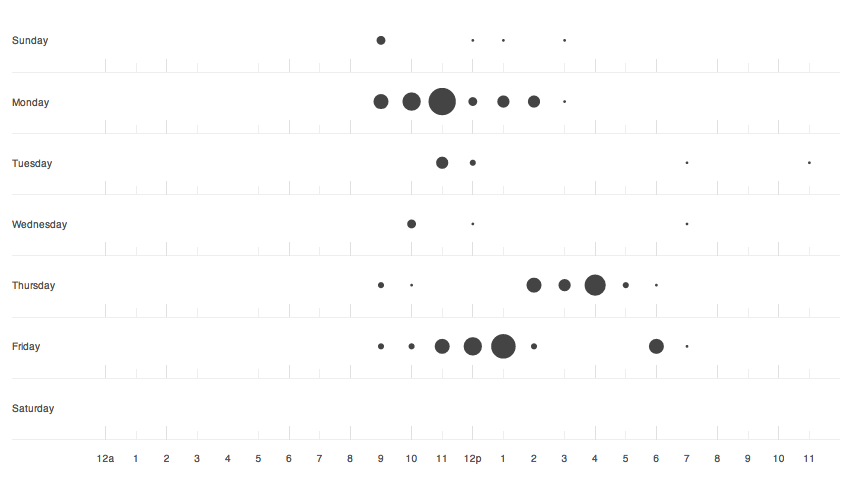
\includegraphics[width=1.0\textwidth]{images/commits.png}
  \caption{Commits by day. Larger circles indicate more commits.}
\end{figure}

% section Process Improvements (end)
\subsubsection{Synchronized source code repository.} % (fold)
\label{ssub:Synchronized source code repository.}

Our Git repository was managed by a single developer(Asger), to audit the legibility of the commits and upon review commits were made by the Git master to keep the repository free from conflicts.
% subsubsection Synchronized source code repository. (end)
\begin{figure}[!ht]
  \centering
    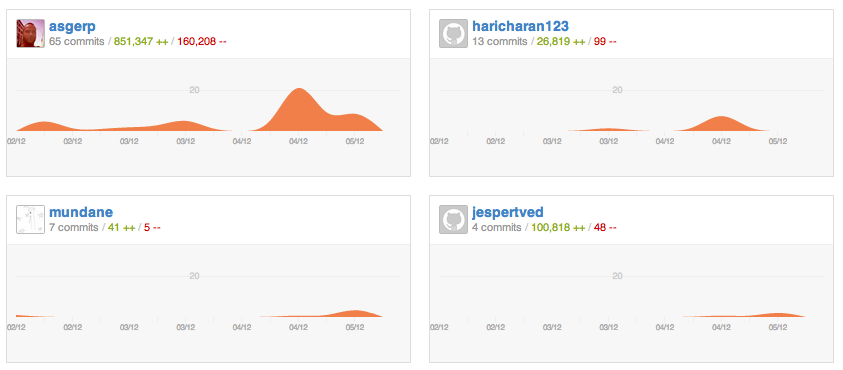
\includegraphics[width=1.0\textwidth]{images/contrib.png}
  \caption{Commits by contributors.}
\end{figure}

Based on the measurements we found we conducted workshop to reflect on the process and identify the key issues. We have  some areas of concern however there were plenty of things that went right too.

\begin{itemize}
	\item	Overall software architecture was insightful and added flexibility to make improvements. Implementation of core functionalities of  the system.
	\item	Synchronized code repository.
	\item	Product testing based on static analysis tool JSLint and Siesta was surprisingly easy.
	\item	A plug-in free pure JavaScript based File Browser.
	\item	Better Sprint Delegation:Better coordination on task and work assignment.
	\item	Refactoring Code:Updated Git with re-factored code.
	\item	Decided on and set up documentation tool for JavaScript.
\end{itemize}

However few tasks some of the processes that needs more attentions were:
\begin{itemize}
	\item Members did not always update the sprint backlog.
	\item We underestimated some tasks and therefore used more time.
	\item Time spent on researching tool and methods.
	\item Consistency in code integration.
	\item We had few physical meetings, as many members are busy with other courses and work.
\end{itemize}

\subsection{Process Change}
There are a number of things we can do to improve processes within the team:
\begin{itemize}
	\item We have to make sure that all members are updating the sprint backlog. We can do this by making it compulsory to update the document, at least, every Monday and Wednesday.
	\item Using SCRUM we hope that the precision of our estimates improve over time, and if thats not the case we can implement estimation guidelines, using expert judgement, experience and task decomposition.
	\item Time spent on researching will decrease as our experience using our tool increase.
	\item Use reverse engineering to increase consistency in code integration.
	\item Make meetings once a week mandatory.
\end{itemize}


\appendix
\section{Scrum Material} % (fold)
\label{sec:Scrum Material}

% section Scrum Material (end)
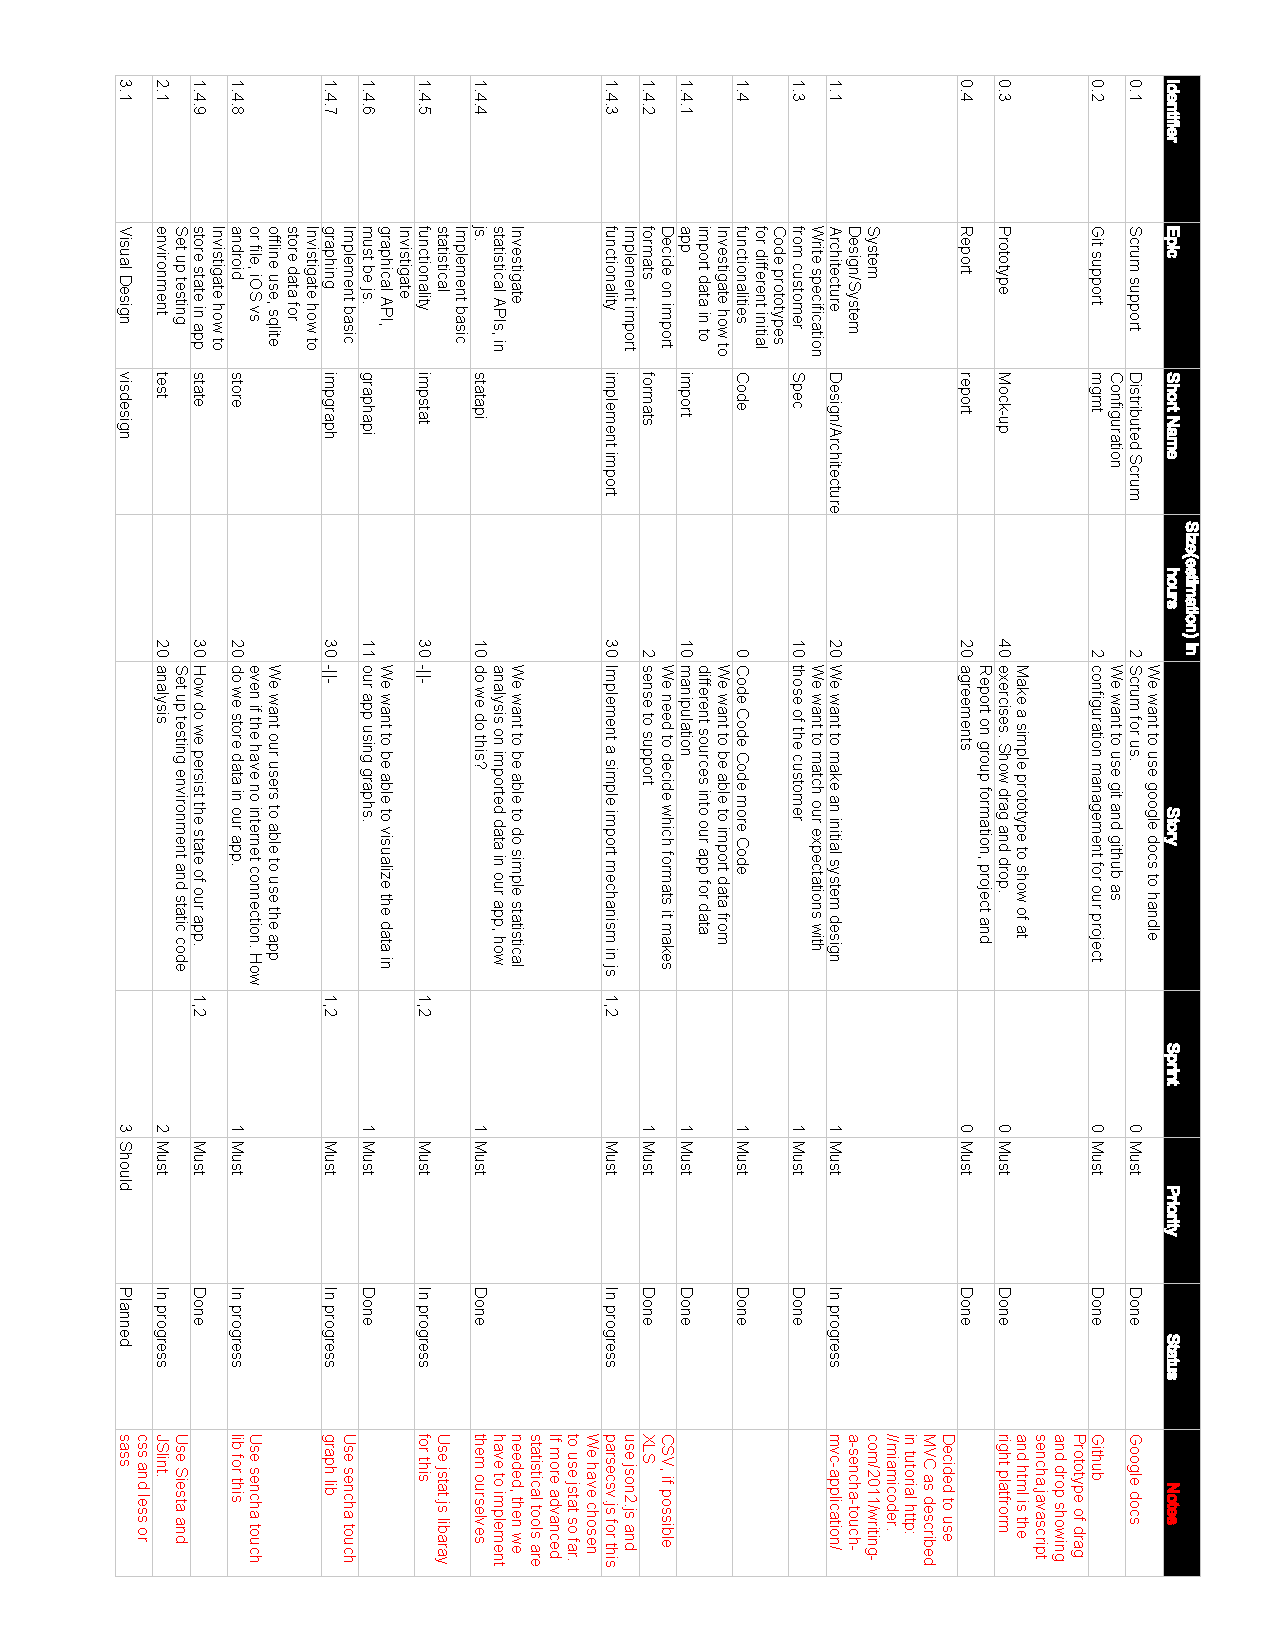
\includepdf[pages={-}]{images/backlog.pdf}
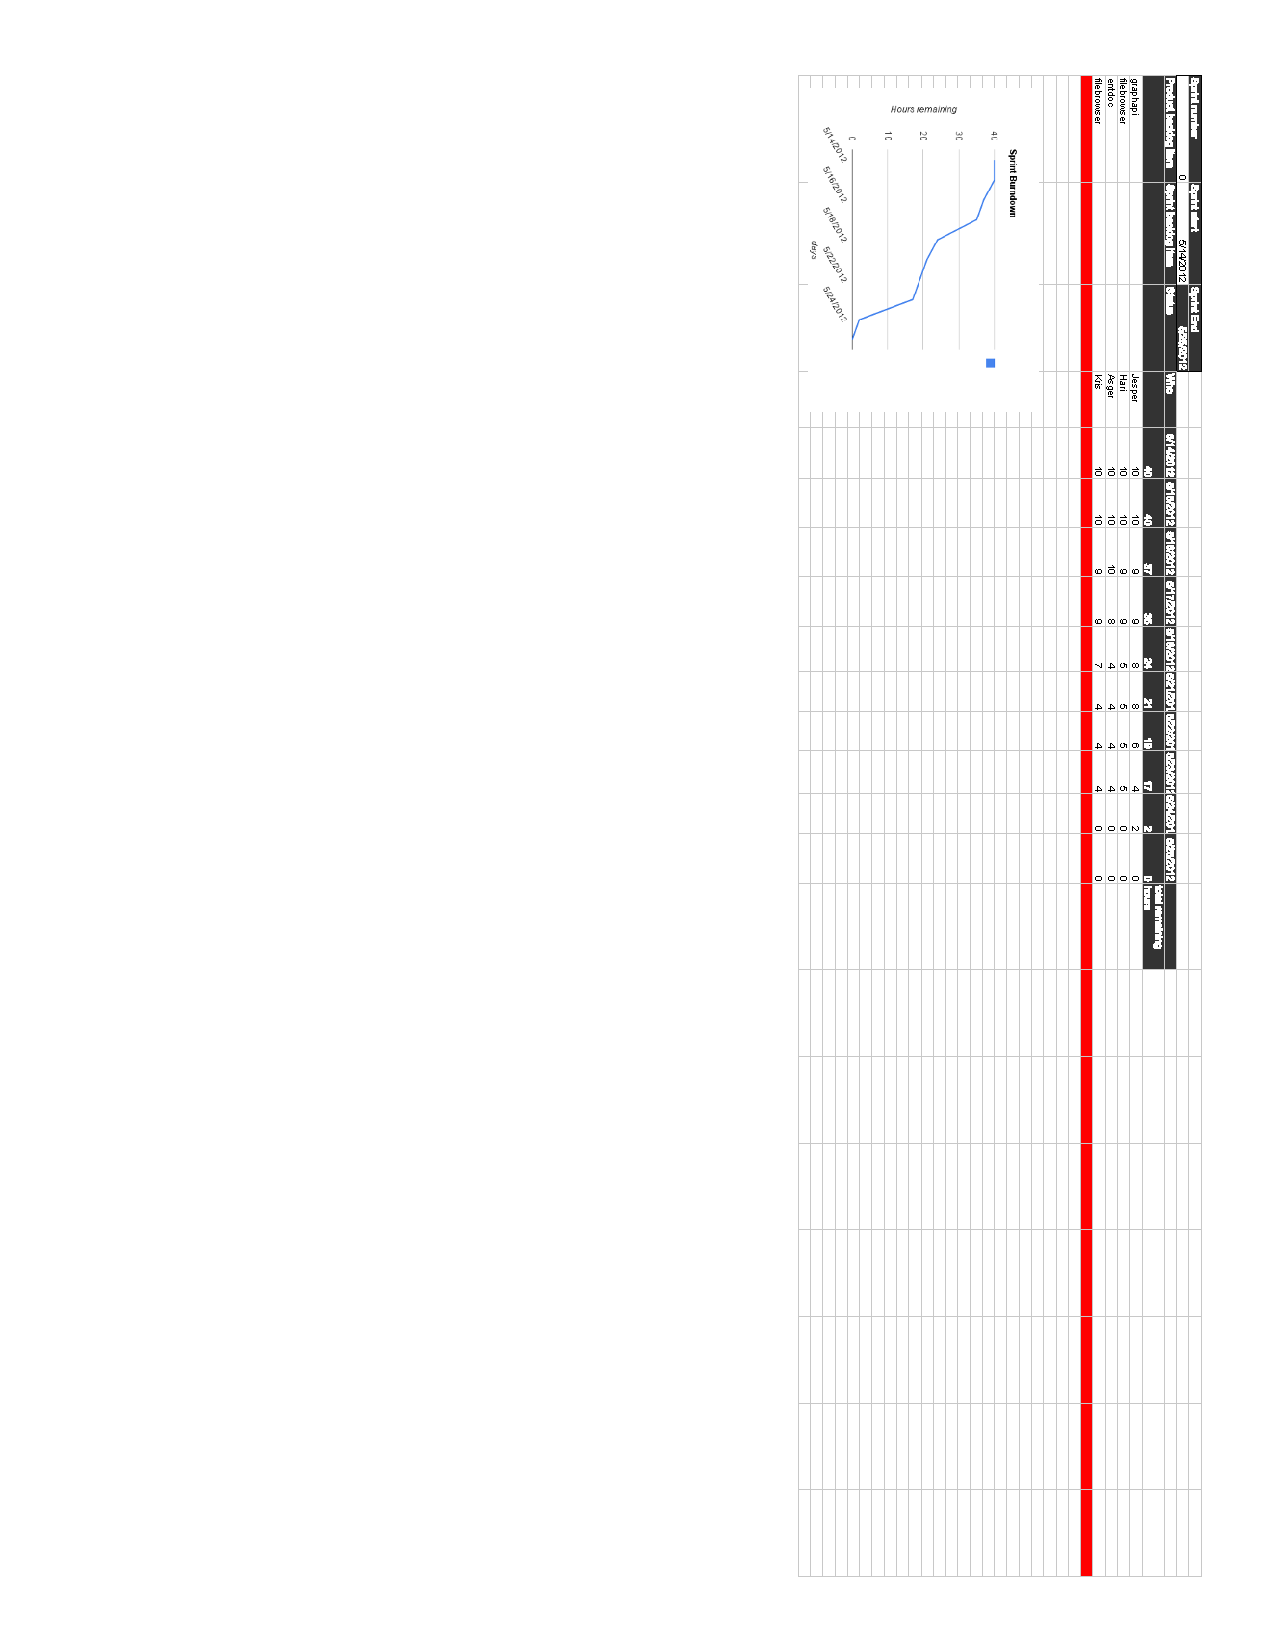
\includepdf[pages={-}]{images/sprint_4.pdf}

\bibliographystyle{plain}
\bibliography{refs}
\end{document}